\documentclass{article}
\usepackage{graphicx} % Required for inserting images
\usepackage{geometry}
\usepackage{circuitikz}
\usepackage{siunitx}
\usepackage{CJKutf8}
\usepackage{amsmath}
\usepackage{amssymb}
\usepackage{caption}
\usepackage{float}
\geometry{top=10mm, left=20mm, a4paper}
\title{STC Networks}
\author{梁程捷(B11901136),吳奕娃(B11901080)}
\date{}

\begin{document}
\begin{CJK*}{UTF8}{bkai}
\maketitle

\section*{Low-Pass RC Circuit}
\begin{minipage}{0.5\textwidth}
\begin{table}[H]
\begin{tabular}{|c|c|c||c|c|c|}
    \hline
    $f$ (\unit{\hertz}) &  $V_i$ (V)& $V_o$ (V) & $f$ (\unit{\hertz}) &  $V_i$ (V)& $V_o$ (V)\\
    \hline\hline
    200	 & 21.2 & 21.2 & 2500 & 20.4 & 11.6  \\
    400  & 21.2 & 20.4  & 3000  & 20.4 & 10.4\\
    600	& 21.2 & 19.6 & 3500 & 20.4 & 9.2\\
    800	& 21.2 & 18.8 & 4000 & 20.4& 8.4\\
    1000& 21.2 & 18.4 & 5000 & 20.4 & 7.2\\
    1100& 21.2 & 17.0 & 6000 & 20.4 & 6.0\\
    1200& 21.2 & 16.6 & 7000& 20.4 & 5.6\\
    1300 & 21.2 & 16.2 & 10000& 20 & 4.4\\
    1400 & 21.2	 & 16.0 & 20000& 20 & 2.8\\
    1500 & 21.2	& 15.2 & 30000 & 20 & 2.4\\
    1600 & 21.2 & 14.8 &  &  & \\
    2000 & 20.4	& 13.2 &  &  & \\
 \hline
\end{tabular}
\caption{low-pass RC raw experimental data}
\end{table}
\end{minipage}\hspace{20mm}
\begin{minipage}{0.5\textwidth}
\begin{figure}[H]
   
    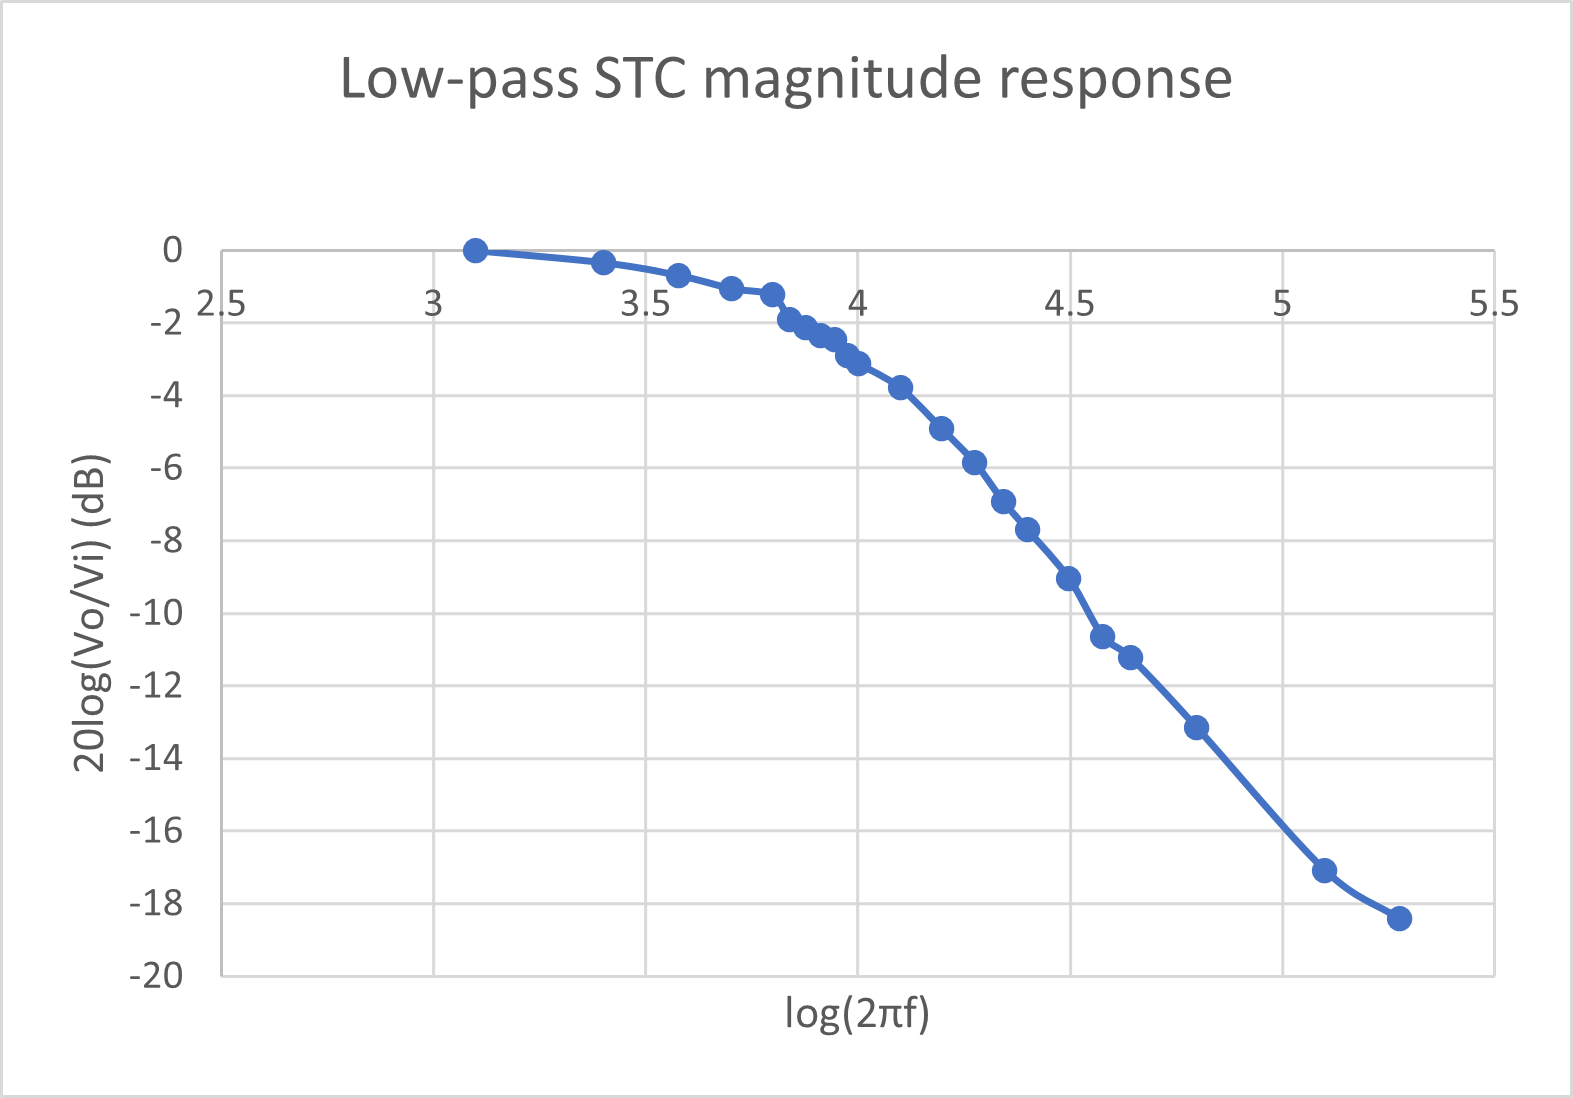
\includegraphics[scale=0.65]{lowpassstc.jpg.png}
    \caption{Low-Pass RC Circuit magnitude response}
\end{figure}
\end{minipage}
\begin{equation*}
    f_{3dB,calculated} = 1591 \,\unit{\hertz},\,f_{3dB,measured} = 1600\,\unit{\hertz}
\end{equation*}

\section*{High-Pass RC Circuit}

\begin{minipage}{0.45\textwidth}
\begin{table}[H]
\begin{tabular}{|c|c|c||c|c|c|}
    \hline
    $f$ (\unit{\hertz}) &  $V_i$ (V)& $V_o$ (V) & $f$ (\unit{\hertz}) &  $V_i$ (V)& $V_o$ (V)\\
    \hline\hline
    100	    & 11.2 & 1.6 & 1800 & 11.0 & 8.0  \\
    1000    & 11.0 & 6.2 & 1900 & 10.8 & 8.2 \\
    1300	& 11.0 & 7 & 2000 & 10.8 & 8.4 \\
    1400	& 11.0 & 7.2 & 3000 & 10.8 & 9.2\\
    1500	& 11.0 & 7.6 & 5000 & 10.6 & 9.6\\
    1600	& 11.0 & 7.6 & 7000 & 10.6 & 10.0\\
    1700	& 11.0 & 7.8 & 10000 & 10.6 & 10.2 \\
 \hline
\end{tabular}
\caption{high-pass RC raw experimental data}
\end{table}    
\end{minipage}\hspace{25mm}
\begin{minipage}{0.45\textwidth}
\begin{figure}[H]
    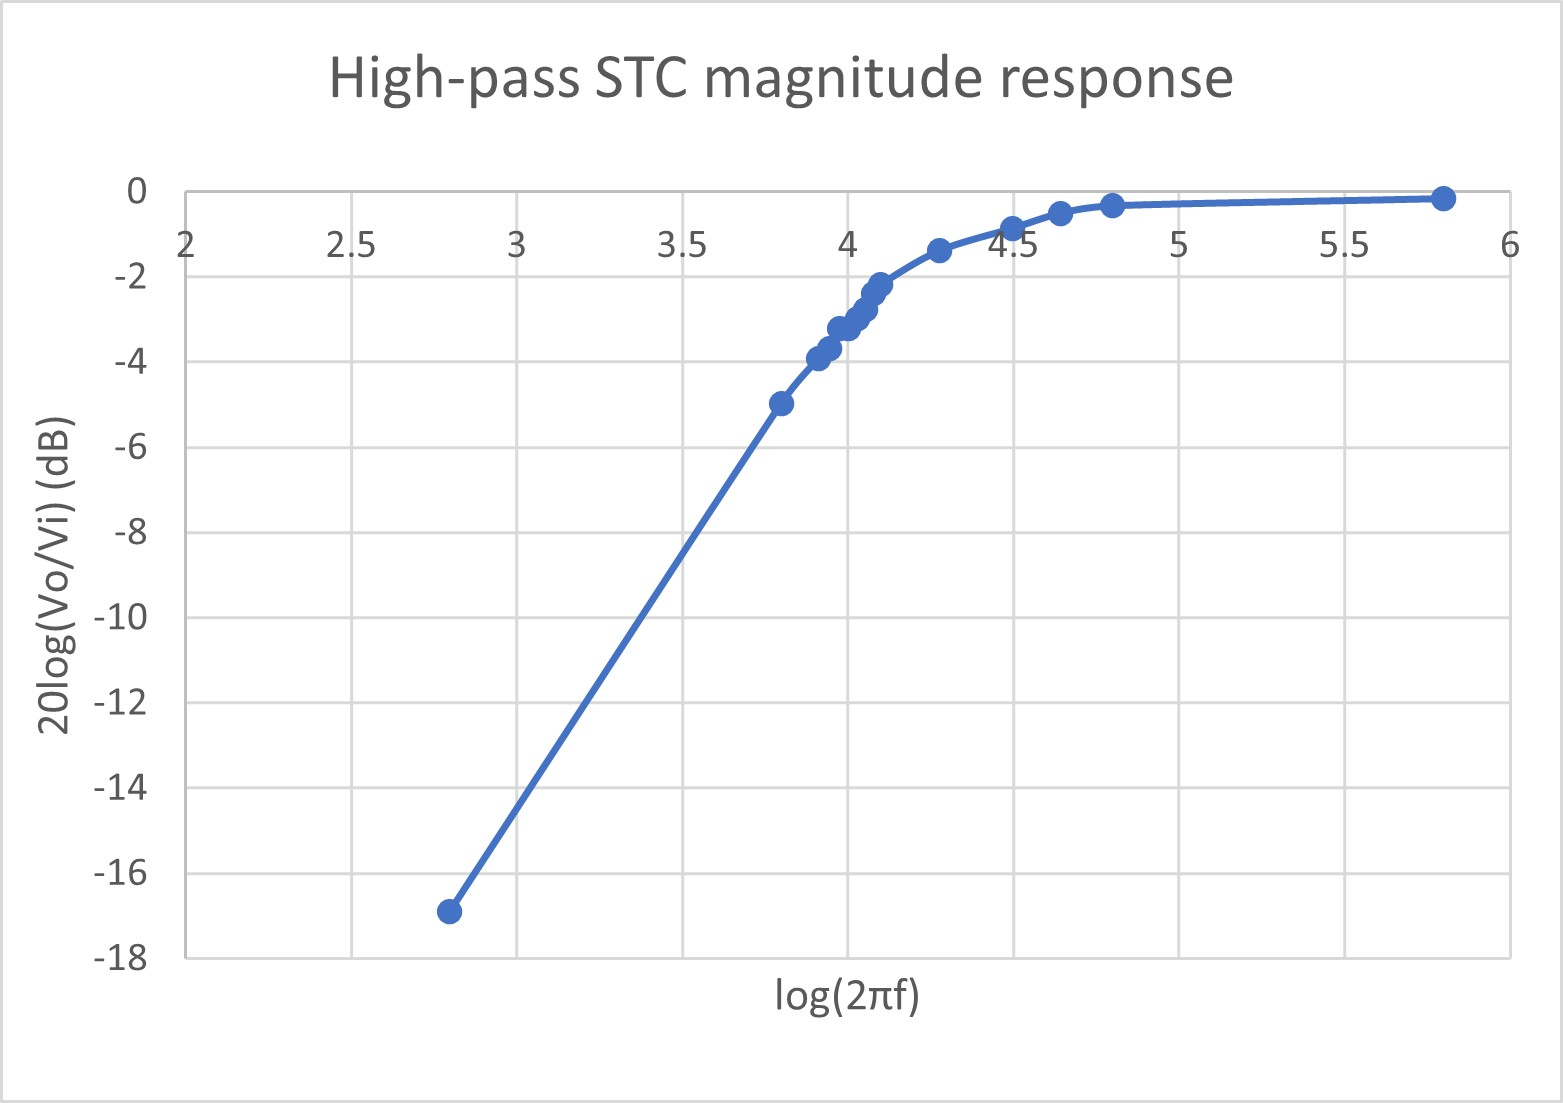
\includegraphics[scale=0.65]{highpassstc.jpg}
    \caption{High-Pass RC circuit magnitude response}
\end{figure}
\end{minipage}
\begin{equation*}
    f_{3dB,calculated} = 1591 \,\unit{\hertz},\,f_{3dB,measured} = 1700\,\unit{\hertz}
\end{equation*}

\section*{Reflection}
我們覺得今天的實驗做得還算順利,振幅在上學期的電路學實驗中做過了,
因此在量取數據上沒有遇到困難,然而我們本來還想嘗試做相位變化的實驗,但是做這個實驗時示波器的數值變化太大難以讀取,最後只好作罷,讓我覺得很可惜。
\end{CJK*}
\end{document}
